\hypertarget{a-budapest-school-tanulokozossegei}{%
\section{A Budapest School
tanulóközösségei}\label{a-budapest-school-tanulokozossegei}}

A Budapest School iskola a gyerekek (családok) és tanárok kisebb
közösségeiből, a \emph{tanulóközösségekből}, áll. Ezek a közösségek
(szervezeti szaknyelven) önálló szervezeti részegységek a nagy
iskolában. A gyerekek szempontjából a tanulóközösség az ő elsődleges
közösségük az iskolán belül, az a biztonságot adó közösségük, ahova
tartozni tudnak és akarnak. A tanárok szempontjából a tanulóközösség egy
belátható gyerek- (család-) közösség, akik a tanulásukért és a jóllétükért
felelősséget tudnak vállalni egy kis tanárcsapattal közösen.

A tanulóközösségek nem osztályok, nem iskolák, nem évfolyamok, nem az
egy telephelyen tanuló gyerekek összessége, hanem a BPS
tanulóközösségei. Jellemző rájuk, hogy

\begin{itemize}
\tightlist
\item
  A tanulóközösségeket a tanulásszervező \emph{tanárcsapatok} vezetik.
\item
  A tanulóközösségek maguk alakítják ki saját szabályaikat,
  normarendszerüket, szokásaikat és kultúrájukat.
\item
  A tanulóközösségek maguk alakítják a tagjaik órarendjét,
  foglalkozásait, és ebben nem kell más tanulóközösségekhez igazodniuk.
\end{itemize}

A tanulóközösségek fogalma eltér az iskolai osztályoktól, mert

\begin{itemize}
\tightlist
\item
  különböző évfolyamon lévő gyerekek tartozhatnak egy közösségbe;
\item
  jellemzően kisebb csoportokban tanulnak a gyerekek, amíg az iskolai
  osztályok elsődleges feladata, hogy az osztály gyerekeit együtt
  tanítsa a tanár.
\end{itemize}

Az Alternatív Közgazdasági Gimnázium \emph{kisiskola} modellje adta
számunkra az elsődleges inspirációt. Az AKG-ban harminc éve a teljes
gimnázium 8 önálló pedagógia műhelyből, a kisiskolákból áll. A kisiskolák
önálló teret kapnak a nagy épületen belül, maguk döntenek a fizikai
térről, van saját tanárcsapatuk és saját szokásaik. Ez a gondolat
keveredett az eredetileg szoftverfejlesztő cégek \emph{agilis csapatok}
fogalmával. A modern cégek olyan kisebb csapatokat hoznak létre a nagy
vállalatban, ahol keresztfunkcionális csoportokban minden eszköz,
szakértelem megvan ahhoz, hogy önállóan terméket hozzanak létre. A
tanulóközösségeket vezető tanárcsapatok agilis csapatoknak tekinthetőek.

\begin{figure}
\centering
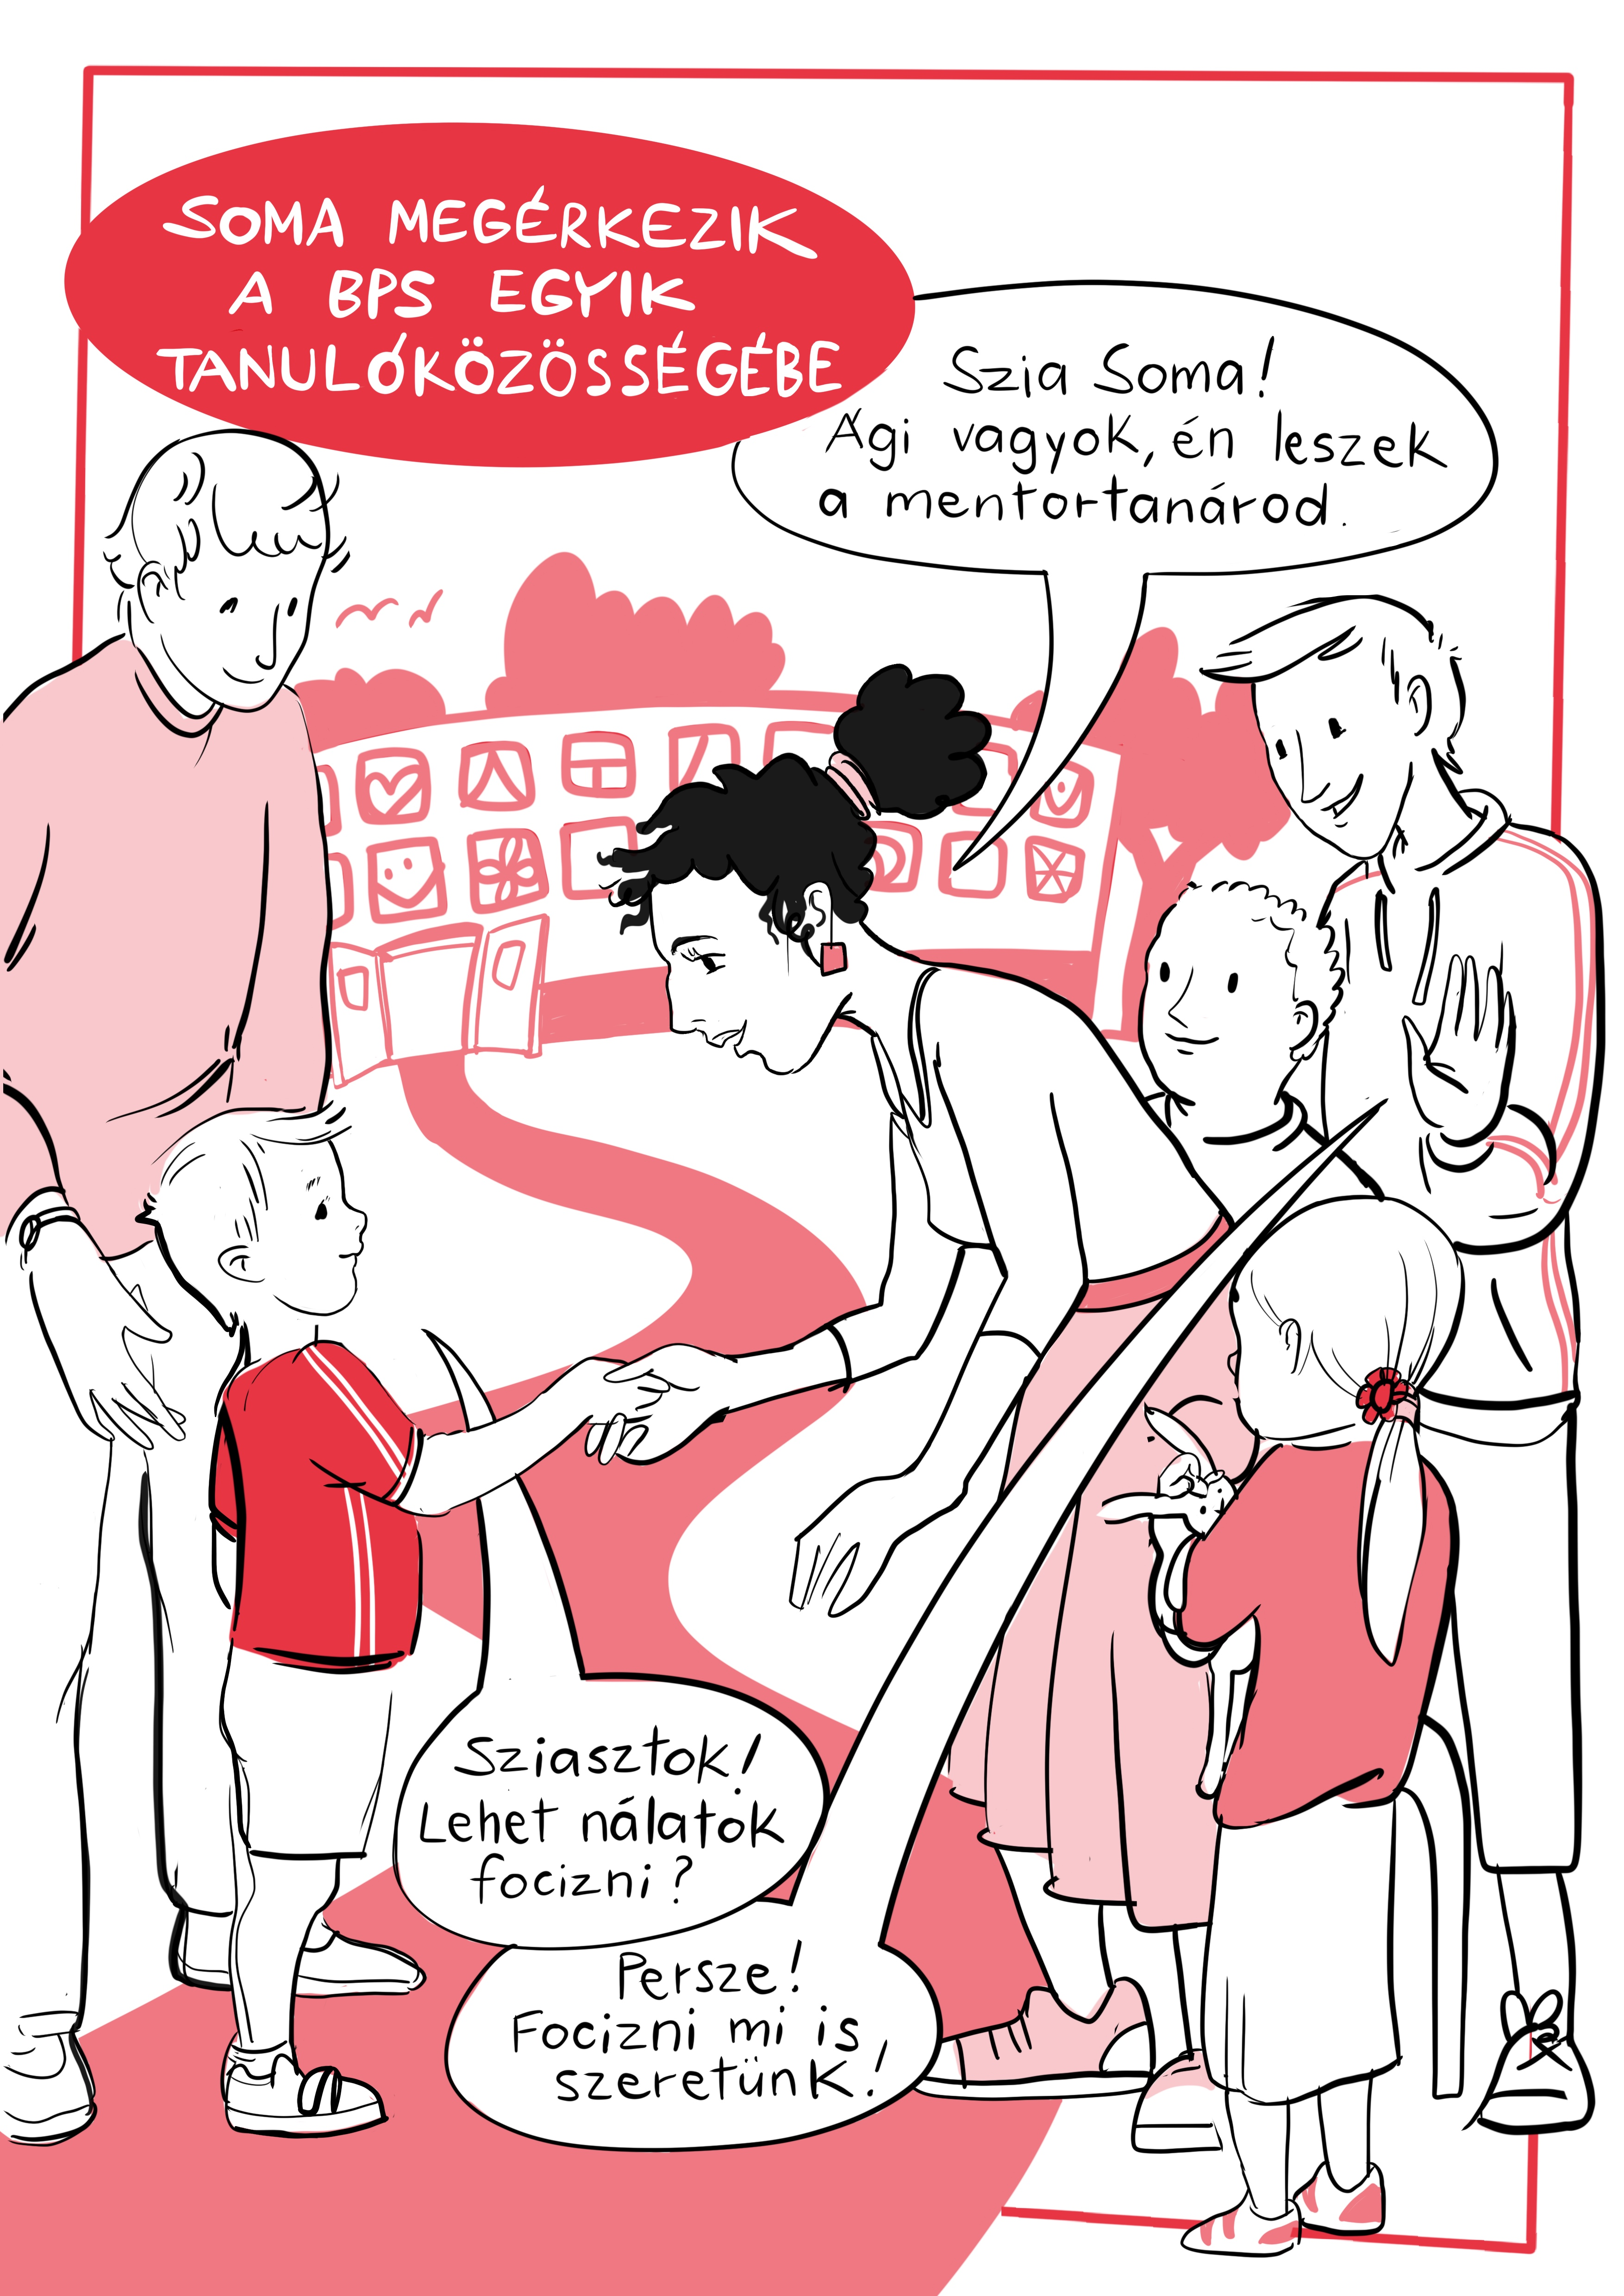
\includegraphics{pics/1a_mikroisk_soma.jpg}
\caption{A tanulóközösség egy gyerek elsődleges közössége.}
\end{figure}

\hypertarget{a-tanulokozossegeket-tanarok-vezetik}{%
\subsubsection{A tanulóközösségeket tanárok
vezetik}\label{a-tanulokozossegeket-tanarok-vezetik}}

A tanulóközösség fontos célja, hogy biztonságot, támogatást nyújtson, és
\emph{így} segítse a közösség tagjainak a minőségi tanulását. A
tanulóközösségeket tanárok irányítják, őket hívjuk tanulásszervezőknek.
Ők felelnek a tanulás tartalmáért, a foglalkozások meghirdetéséért és a
tanulási eredmények nyomon követéséért. Ők döntenek arról, hogy ki és
milyen feltétellel lehet tagja a közösségnek.

\hypertarget{a-tanulokozosseg-allando-a-gyerekek-es-a-tanarok-fluktuacioja-lehetseges}{%
\subsubsection{A tanulóközösség állandó, a gyerekek és a tanárok
fluktuációja
lehetséges}\label{a-tanulokozosseg-allando-a-gyerekek-es-a-tanarok-fluktuacioja-lehetseges}}

A tanulásszervező tanárok vagy gyerekek kilépése a tanulóközösség
fennállását nem érinti, helyettük a tanulóközösség új tanulásszervező
tanárt és gyereket vehet fel.

A tanulóközösség létrehozásakor arra kell törekedni, hogy olyan gyerekek
tanuljanak együtt, akik támogatni tudják egymást a tanulásban. A
gyerekek mindaddig a tanulóközösség tagjai, amíg ott jól tudnak tanulni,
és a közösség és a gyerek kapcsolata gyümölcsöző.

\begin{figure}
\centering
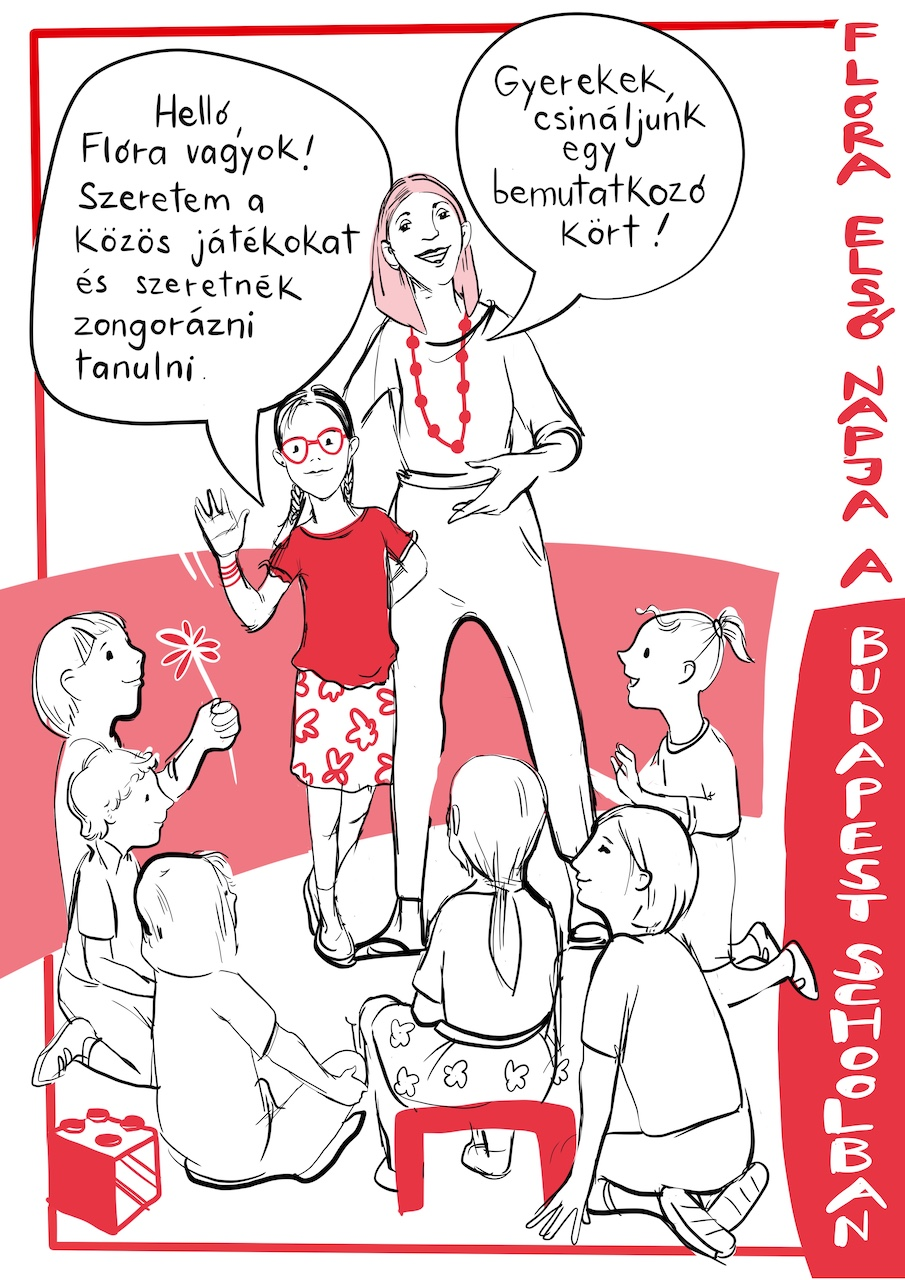
\includegraphics{pics/1b_mikroisk_flora.jpg}
\caption{A tanulóközösség egy családias közösség.}
\end{figure}

\hypertarget{a-tanulokozossegeknek-sajat-fokuszuk-helyszinuk-stilusuk-alakulhat-ki}{%
\subsubsection{A tanulóközösségeknek saját fókuszuk, helyszínük,
stílusuk alakulhat
ki}\label{a-tanulokozossegeknek-sajat-fokuszuk-helyszinuk-stilusuk-alakulhat-ki}}

A tanulóközösségek nemcsak abban térnek el egymástól, hogy kevert
korcsoportban, más korosztályú gyerekek, más érdeklődések mentén, és ily
módon más célokat követve tanulnak, hanem területileg, regionálisan is
eltérőek lehetnek.

A tanulóközösség-rendszerben lehetőség van arra, hogy adott tanulási
környezetben úgy váltakozhassanak a hangsúlyok a csoport és az egyén
érdeklődését követve, hogy közben fennmaradjon a tanulási egyensúly a
tantárgyak között. Ezért a tanulóközösségek órarendje, alkalmazott
pedagógiai módszerei, a tantárgyak összevonásának módja eltérő lehet.

Van olyan tanulóközösség, amely a fejlesztési célok eléréséhez és a
saját célok mentén már 6 éves gyerekek tanulásánál a robotika eszközeit
használja, másutt drámafoglalkozásokkal fejlesztik 12 éves gyerekek a
szövegértésüket és éntudatukat.

\hypertarget{a-tanulokozossegekben-a-gyerekek-nagymertekben-befolyasoljak-hogy-mit-es-hogyan-tanulnak-es-alkotnak}{%
\subsubsection{A tanulóközösségekben a gyerekek nagymértékben
befolyásol\\-
ják, hogy mit és hogyan tanulnak és
alkotnak}\label{a-tanulokozossegekben-a-gyerekek-nagymertekben-befolyasoljak-hogy-mit-es-hogyan-tanulnak-es-alkotnak}}

A tanulóközösségekben (a tanulásszervezők által meghatározott kereteken
belül) megfér egymással több, különböző saját céllal rendelkező gyerek
addig, amíg a tanulásszervezők minden gyerek számára biztosítani tudják
a tantárgyak által meghatározott tanulási eredmények elérését.

A tanulásszervezők feladata és felelőssége, hogy olyan közösségeket
építsenek, amelyek kellően diverzek, és mégis jól működnek. A
közösségnek a gyerekek igényeit és a NAT céljait egyaránt ki kell
elégítenie.

A tanulásszervezők választási lehetőségeket kínálnak (azaz modulokat
dolgoznak ki), amikből a gyerekek (a mentoruk és szüleik segítségével) a
saját céljaikat, érdeklődésüket leginkább támogató saját tanulási tervet
és utat alkotnak.

Eltérhet, hogy egy-egy gyerek mit tanul, ezért az is, hogy mikor és
hogyan sajátítja el a szükséges ismereteket: egy közösségben megfér a
központi felvételire fókuszáló 11 éves gyerek, és aki ekkor inkább a
Mi\-ne\-craft programozásában akar elmélyedni, ezért más képességek
fejlesztésével lassabban halad.

\hypertarget{csatlakozas-a-tanulokozossegekhez}{%
\subsubsection{Csatlakozás a
tanulóközösségekhez}\label{csatlakozas-a-tanulokozossegekhez}}

Arról, hogy egy gyerek csatlakozhat-e egy tanulóközösség közösségéhez, a
tanulásszervezők döntenek, figyelembe véve a gyerek életkorát, a
közösségben való eligazodását, érdeklődését, saját fejlődési igényét. A
kiválasztás fő elve, hogy a közösség fejlődjön minden gyerek
csatlakozásával.

\hypertarget{tanulokozossegek-osztalyai-es-csoportbontasai}{%
\subsection{Tanulóközösségek osztályai és
csoportbontásai}\label{tanulokozossegek-osztalyai-es-csoportbontasai}}

Egy tanulóközösségek minimális létszáma hat, maximális létszáma 60 fő, és
a tagok évfolyamszintje között maximum hat évfolyam lehet. Egy
tanulóközösségbe több osztály gyerekei tartozhatnak, de a
tanulóközösségek nem tekinthetőek összevont osztályoknak. Az egy
osztályba tartozó gyerekek tanulási célja nagyon hasonló, az évfolyamhoz
tartozó tanulási eredményeket el szeretnék érni.

A BPS mindennapjaiban a gyerekek a közösségeknél és az osztályoknál
nagyobb csoportban is tanulhatnak.

A tanulóközösségekben az idő legnagyobb részében a közösséget kisebb
csoportokra bontják a tanulásszervezők, hogy a tanulás hatékonyabb legyen.

\begin{itemize}
\tightlist
\item
  Egyes foglalkozások vagy modulok (tanulási-tanítási egységek) során
  egy-egy projektre szerveződnek, ilyenkor általában az eltérő képességű
  és életkorú gyerekek is kitűnően tudnak együtt dolgozni.
\item
  Más foglalkozások vagy modulok esetén a csoportokat a tanár
  képességszint alapján hozza létre. Ilyen csoportok lehetnek a
  másodfokú egyenletek megoldóképletét megismerő csoport, az írni
  tanulók csoportja, vagy egy angol nyelvű újság szerkesztésére és
  megírására alakult modul, ahol a nyelvismeretnek és a szövegalkotási
  képességnek már egy olyan szintjén kell állni, hogy a projektnek jól
  mérhető kimenete lehessen.
\item
  Vannak olyan foglalkozások és tanulási modulok, amikor kifejezetten az
  egy évfolyamra járó gyerekek tanulnak együtt, mert például a 9.
  évfolyamos matematikatanulási eredmények elérésén dolgoznak.
\end{itemize}

Több szintje van a csoportmunkának.

\begin{enumerate}
\def\labelenumi{\arabic{enumi}.}
\tightlist
\item
  A tanulóközösség közössége heti rendszerességgel tarthat
  iskolagyűlést, fórumot, plenárist, iskolakonferenciát. Ilyenkor a
  tanulóközösség közössége dolgozik együtt.
\item
  Egy tanulási modul csoportjának rendezőelve lehet:

  \begin{enumerate}
  \def\labelenumii{\alph{enumii}.}
  \tightlist
  \item
    egy képességszinten lévő gyerekek tanulnak együtt;
  \item
    a közös érdeklődés hozza össze a csoporttagokat;
  \item
    direkt a véletlenszerűségben van az érdekesség, mert keveredni
    akarnak;
  \item
    kölcsönös szimpátia és vonzalom a modultagok között: most azért
    vannak egy csoportban, mert egy csoportban akartak lenni.
  \end{enumerate}
\item
  Egy-egy foglalkozáson belül is sokszor csoportot alkotunk, az előző
  elvek alapján.
\end{enumerate}

Arra is lehetőség van, hogy egy csoport tagjai több tanulóközösség
tagjaiból álljanak össze, ha az támogatja a tanulást és az utazás
biztonságosan megoldható.
